\chapter{Reinforcement Learning Approach}
\label{chap:reinforcementlearning}
This chapter describes a \ac{RL} approach, used to tackle the important problem of optimized trade execution. To a large extend, it is based on the \ac{RL} formulation, as described by Nevmyvaka \etal \cite{Nevmyvaka:2006}. Q-learning and dynamic programming are fused to find an optimal, state-based strategy from a training set of historic orderbook date. Sampling the discretized state space\footnote{The state space describes actual trade progress (\ie \emph{remaining time} and \emph{remaining inventory}) as well as current market situation.} in a brute force manner, the authors achieved an impressive 50\% gain over the more simple Submit \& Leave Strategy (see \Cref{chap:tradingstrategies}).\\

Some of the assumptions made in the original approach deserve a discussion and leave room for potential improvements. As their work was based on a rather large, proprietary dataset of 1.5 years of millisecond time-scale limit order data from \acs{NASDAQ}, it was furthermore intriguing to evaluate its performance on a smaller, self-recorded dataset of limited resolution.


\section{General Framework}
\label{chap:reinforcementlearning:original}
x


\subsection{State space}
\label{chap:statespace}
The state space consists of various variables, describing the current trade progress (\emph{private variables}) and the current market situation as observable from orderbook data (\emph{market variables}). The two private variables \emph{remaining time} (\lstinline!time!) and \emph{remaining inventory} (\lstinline!volume!) make the base for all subsequent experiments, while optional market variables may be enclosed to potentially assist the process of decision finding.\\

Each \lstinline!state! $s \in <time, volume ,o_1, o_2, ...>$ forms a vector of at least both private variables, plus a variable number of market variables. More specifically, the following market variables were evaluated in terms of improvement over a state space based on two private variables only.
\begin{description}
\item[Bid-Ask Spread]: spread between best bid price and best ask price.
\item[Bid-Ask Volume Misbalance]: volume imbalance between orders at the best bid price and the best ask price.
\item[Immediate Market Order Cost]: costs, if remaining volume would be executed immediately, at the current market price.
\item[Signed Transaction Volume]: signed volume of all trades executed within last 15 seconds. A positive value indicates more buy orders, while a negative value complies to more sell orders being executed.
\end{description}

In the original approach, market variables were discretized into 0 (low), 1 (medium) and 2 (high), while the concrete category mapping process was not further described. Market variables are extracted from the original orderbooks, as if the market had evolved without our impact. Private variables where discretized in 4 to 8 bins, while greater resolutions led to strictly better results and linearily higher computation times.

\subsection{Action space}
\label{chap:actionspace}
Actions define the level of trading aggression to be performed. In the original approach, action $a \in \mathbb{R}$ defines the deviation between current best price and chosen limit price, as $bid + a$ (for buy orders) and $ask - a$ (for sell orders). As such, actions must cross the full bid-ask-spread to find matching orders in the opposing book. Large actions $a$ result in larger fractions of the order volume being matched immediately. Smaller or even negative actions $a$ help to prolong the actual execution, and may help to profit from opportune market movements.\\

In case of the market situation as shown in \Cref{table:orderbook:example:again}, a buy order with an aggressive action $a=1.4$ would map into $limit=bid+a=28.7+1.4=30.1$. This limit would allow trading up to 75 shares instantaneously.\\

\begin{table}
\centering
\begin{tabular}{lrlrrr}
\toprule
{} &  Amount &    Type &  Volume &  VolumeAcc &  norm\_Price \\
\midrule
31.00 &   200.0 &     ask &  6200.0 &     8425.0 &    1.074533 \\
30.00 &    50.0 &     ask &  1500.0 &     2225.0 &    1.039871 \\
29.00 &    25.0 &     ask &   725.0 &      725.0 &    1.005208 \\
28.85 &     NaN &  center &     NaN &        NaN &         NaN \\
28.70 &   200.0 &     bid &  5740.0 &     5740.0 &    0.994810 \\
28.50 &   100.0 &     bid &  2850.0 &     8590.0 &    0.987877 \\
28.00 &   300.0 &     bid &  8400.0 &    16990.0 &    0.970546 \\
\bottomrule
\end{tabular}
\caption{Action $a=1.4$ translates into $limit=28.7 + 1.4 = 30.1$.}
\label{table:orderbook:example:again}
\end{table}

The employed number of selectable actions and their actual value range was not further specified.


\subsection{Costs}
\label{chap:costs}
Costs are defined as the slippage induced from the previously chosen actions. The baseline is given by the initial center price. The following formula is used to compute (partial) costs in terms of price deviation from the idealized case of buying all shares at the initial center price:
\begin{equation}
\label{eq:imcost}
   cost_{im} = (avg\_paid - initial\_center) * volume\_traded
\end{equation}
\begin{equation}
   initial\_center = (\dfrac{ask_t+bid_t)}{2} | t=0
\end{equation}

Since the complete trade execution happens within a finite time horizon and full execution of the \lstinline!volume! is mandatory, partial costs can simply be summed up without any discounting. Utilizing the \ac{OTS}, it is not possible to compute occurring costs in advance exactly, as they depend on how the market evolves within the subsequent \lstinline!trading_period!.


\section{Backward learning}
\label{chap:backwardlearning}
In order to learn the optimal limit for each possible situation, orderbook windows are examined in a backward, brute-force manner as described in \Cref{lst:bruteforce:pseudocode}. Each orderbook window from the training data set is sampled $T*I*L$ times, where $T$ is the number of performed limit revisions, $I$ is the number of discrete volume states and $L$ is the number of available actions.

\begin{lstlisting}[frame=single, breaklines=true, basicstyle=\scriptsize, caption=Brute-Force strategy learning approach as described in \Cite{Nevmyvaka:2006}., label=lst:bruteforce:pseudocode]
Optimal_strategy(V, H, T, I, L)
    For t=1 to T
        While(not end of data)
            Transform (orderbook) -> o_1 ... o_R
            For i =0 to I
                For a = 0 to L
                    Set x = [t, i, o_1, ..., o_R]
                    Simulate transition x -> y
                    Calculate immediate cost_im(x, a)
                    Look up argmax cost(y, p)
                    Update cost([t, v, o_1, ..., o_R], a)
    Select the highest-payout action argmax cost(y, p) in every state y to output optimal policy
\end{lstlisting}

While the algorithms running time depends solely on the resolution of the two private variables, the chosen action space and the size of the training data set, it is approximately independent of the number of market variables chosen. The precise transition simulation was not further described, but for this thesis the model described in \Cref{chap:tradeexecution} is utilized. The cost update rule is given below: 
\begin{equation}\label{eq:costfunction}
   cost(x_t, a) = \dfrac{n}{n+1} cost(x_t, a) + \dfrac{1}{n+1} [cost_{im}(x_t,a) + \arg\min_{p}cost(x_{t-1}, p)]
\end{equation}

The algorithm assumes the individual trading\_periods to be of an (approximately) Markovian nature, where the optimal action to choose at state $x_t$ with $t = \tau$ is completely independent of actions chosen previously ($t \geq \tau$).\\

As such, the state-action function can be computed inductively via dynamic programming. In a first round, expected costs for all actions in states being immediate predecessors of end states (\ie $t=1$) are computed according to \Cref{eq:costfunction}. \Cref{fig:heatmap:t1} visualizes the resulting optimal costs (right) and corresponding actions (left) after the first round has finished.

\begin{figure}[ht]
	\centering
   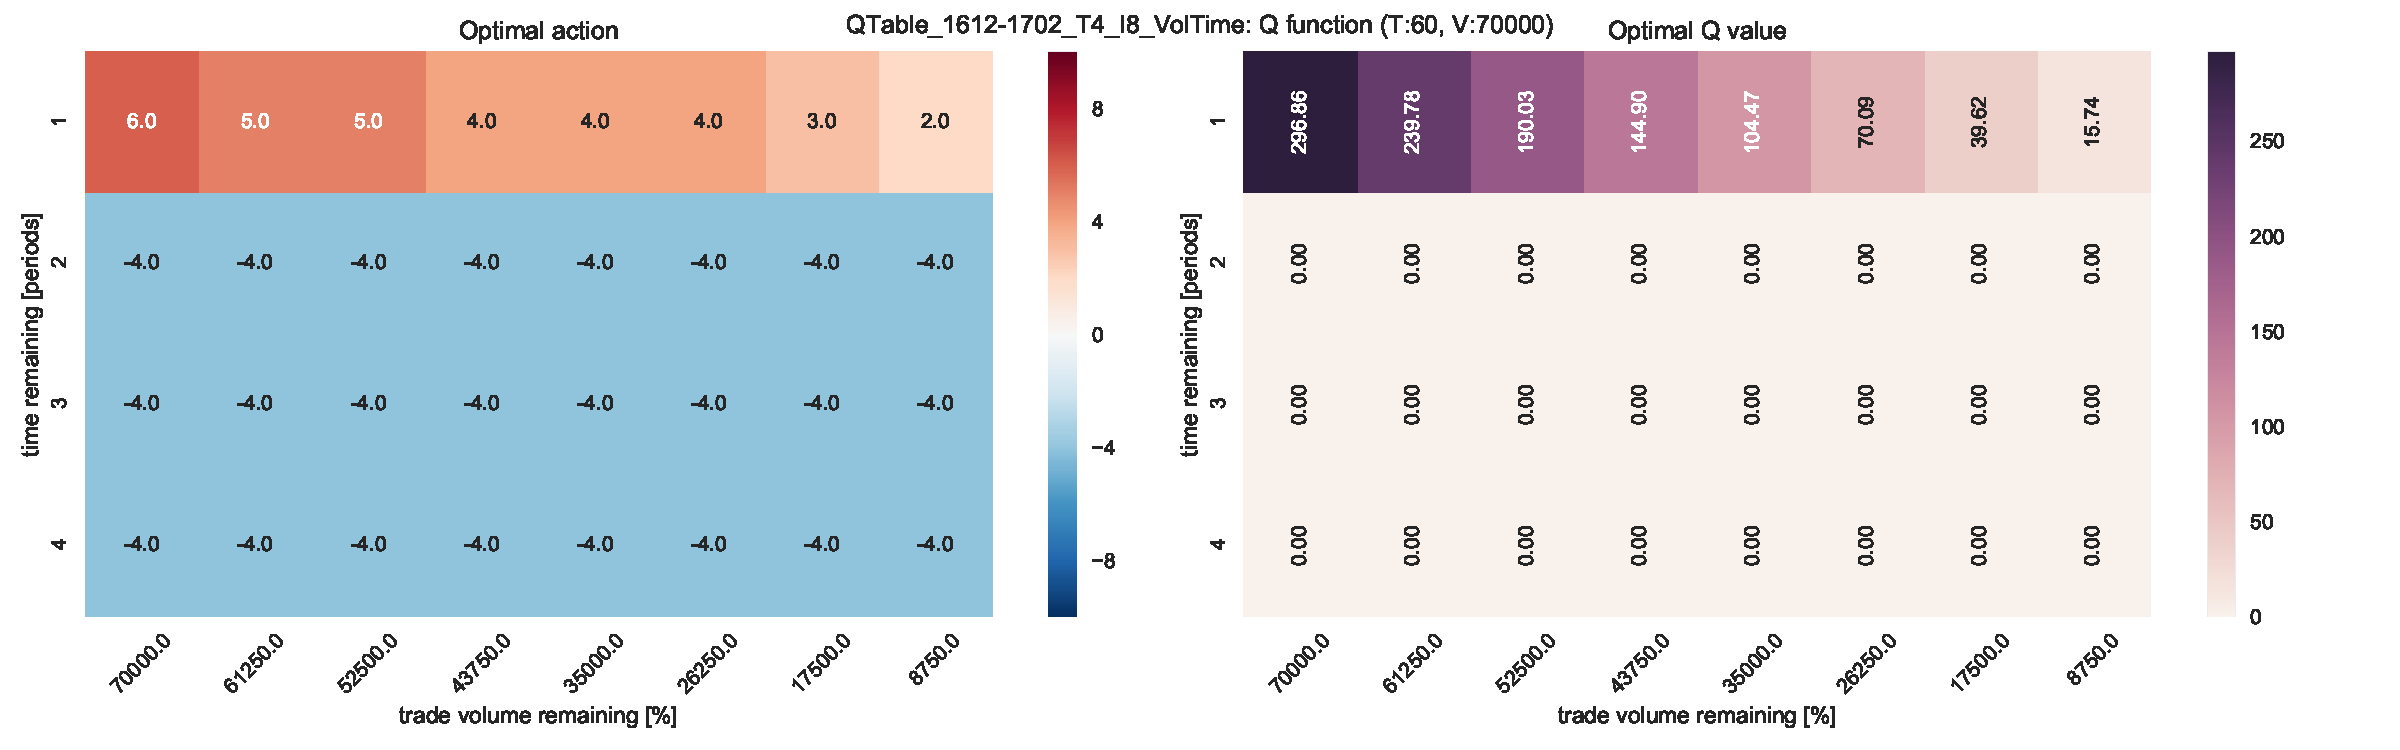
\includegraphics[width=0.8\textwidth]{content/drawings/heatmap_3months_t1}
	\caption{State-Action function, visualized after the first training round.}
	$T=4$, $I=8$, L=15
	\label{fig:heatmap:t1}
\end{figure}

Knowing the optimal state-action values for all states with $t=1$, all informations are given to compute the optimal state-action values for their predecessor states with $t=2$ (see \Cref{fig:heatmap:t2}).

\begin{figure}[ht]
	\centering
   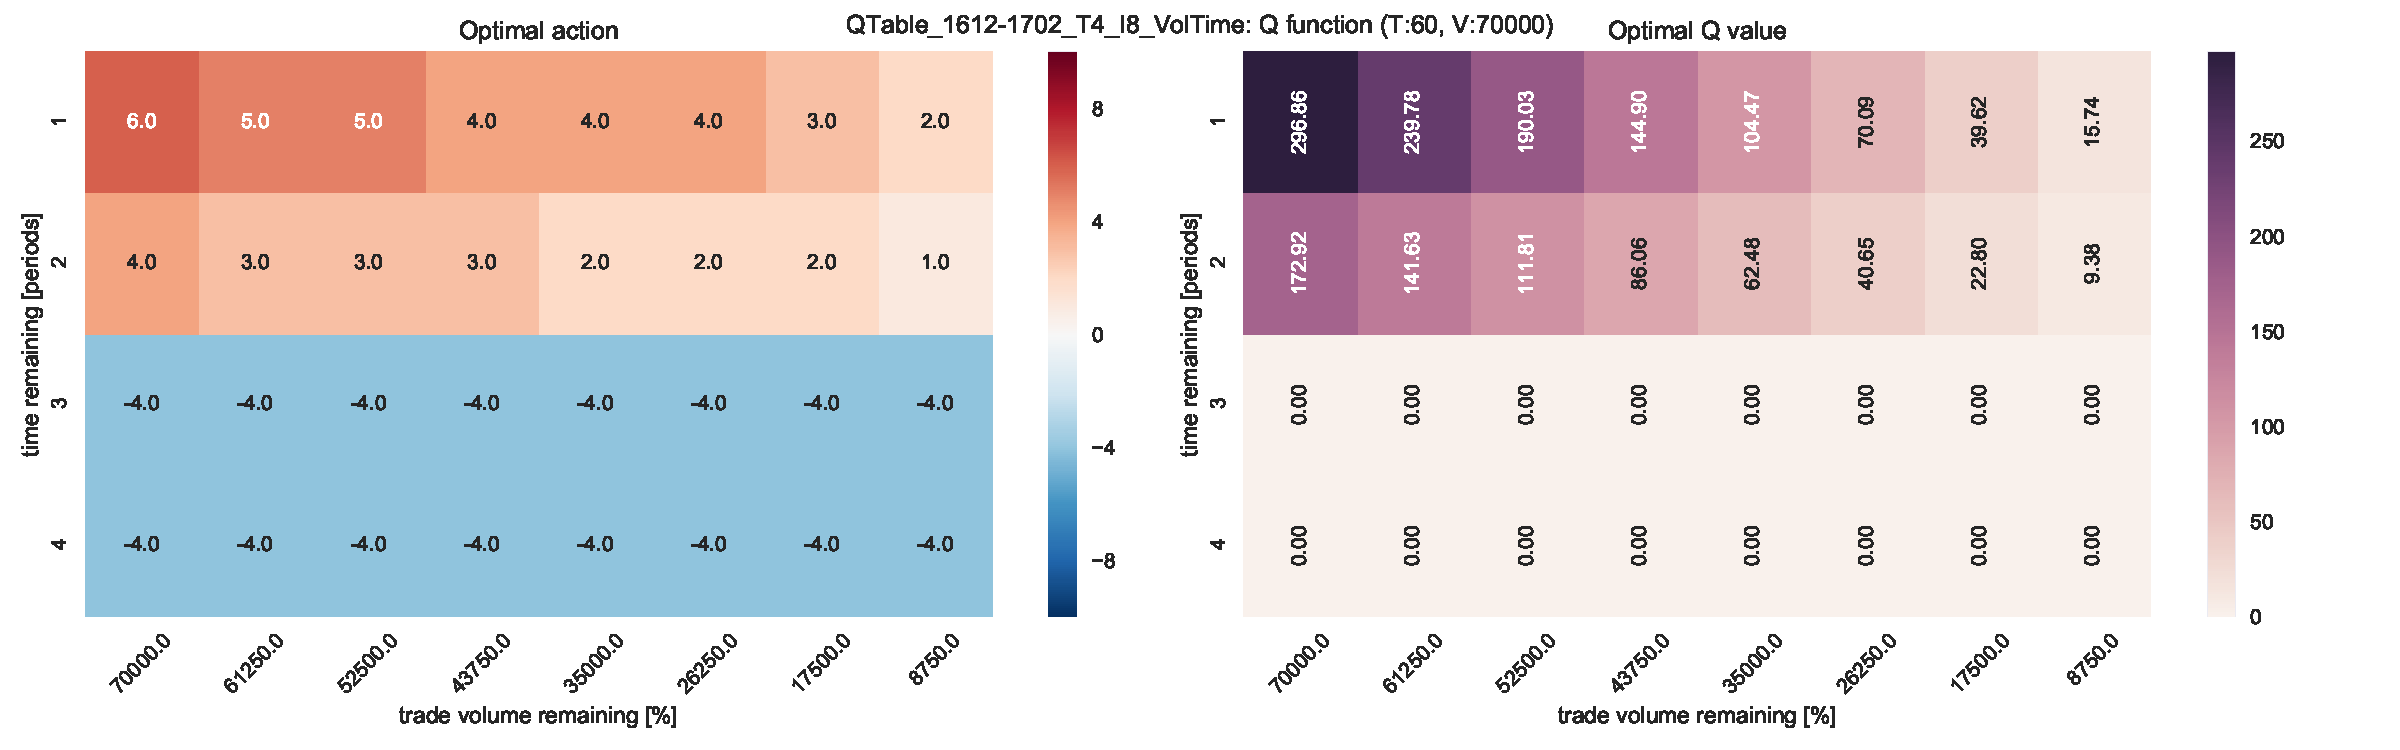
\includegraphics[width=0.8\textwidth]{content/drawings/heatmap_3months_t2}
	\caption{State-Action function, visualized after the second training round.}
	$T=4$, $I=8$, L=15
	\label{fig:heatmap:t2}
\end{figure}

After $T$ iterations a globally optimal policy, as shown in \Cref{fig:heatmap}, has been found. The annotated q values (right) denote the corresponding minimum over all available actions. The visualized state-action function was trained over orderbook snapshots from Nov, 10th 2017 10am to May, 31st 2017, partitioned into 4.154 orderbook windows of 60 minutes length each. Over a trading horizon of $T=4$ \lstinline!trading_periods!, $70.000\$$ cash (discretized in $I=8$ intervals) had to be traded into Bitcoins. The state space included the two private variables \lstinline!time! and \lstinline!volume! only, while the action space comprised $L=15$ actions. As such, a total of $4.154 * 4 * 8 * 15 = 1.993.920$ transition tuples were generated.\\

\begin{figure}[ht]
	\centering
   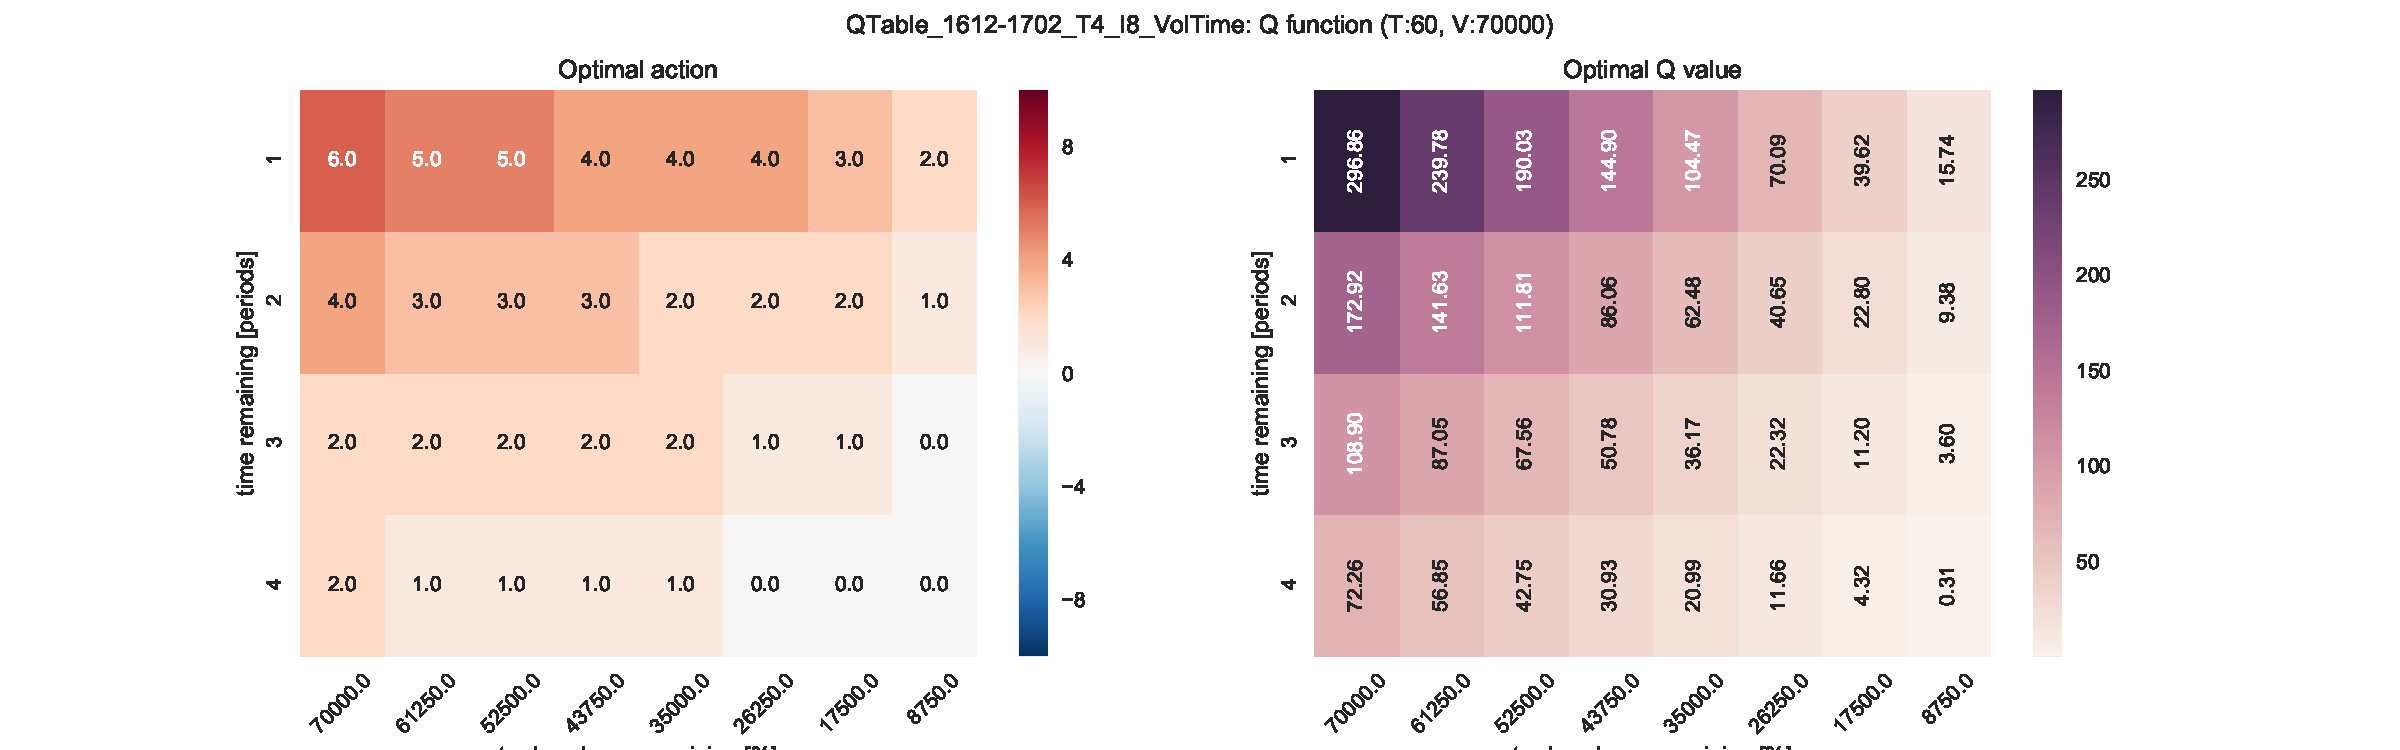
\includegraphics[width=1.\textwidth]{content/drawings/heatmap_3months}
	\caption{Final State-Action function.}
	$T=4$ (60min), $I=8$ (70.000\$), L=15 ([-4, -3, \ldots{}, 9, 10])
	\label{fig:heatmap}
\end{figure}

\Cref{fig:heatmap} illustrates clearly, how the optimal strategy becomes more aggressive as time ceases and a large portion of the trading volume remains unexecuted.




\section{Forward learning}
\label{chap:forwardlearning}

\subsection{Forward Sampling \& Learning}
In order to collect more realistic transition samples (see subsequent discussion in \Cref{chap:backwardalgorithm:discussion:markovianassumption}), an alternative, \emph{forward sampling} method is presented.\\

Rather than examining all available actions on the great variety of combinational possibilities the state space has to offer, the forward approach repeatedly simulates trades in their entirety. The once again utilized \ac{OTS} starts always with $V=100\%$ and keeps going until the full trade is executed. As such, sample transitions stem from a more natural and furthermore fully continuous environment. Only actually attainable states, that could arise in the (simulated) reality, are used as transition start points, potentially increasing their significance. As major disadvantage, this forward sampling approach does not assure exhaustive exploration of the state space. A thorough exploration is not self-evident and must be supervised.\\

The pseudo-code of the forward approach is shown in \Cref{lst:forward:pseudocode}. The algorithm iterates over the training data 

\begin{lstlisting}[frame=single, breaklines=true, basicstyle=\scriptsize, caption=Forward sampling approach., label=lst:forward:pseudocode]
collect_samples_forward(V, H, T, I, L, e)
    While(not end of data)
        init OTS with V=100%
            For epoch=0 to e
                reset OTS at random startpoint
	            Transform (orderbook) -> o_1 ... o_R
	            Apply e-greedy strategy until V=0%
		    Store samples in DataFrame
        occasionally retrain strategy with new collected samples (+ experience replay)
\end{lstlisting}






\section{Discussion}
\label{chap:backwardalgorithm:discussion}
While the presented algorithm exploits the available data profoundly in a brute force manner, the underlying assumptions deserve a short discussion. Alternative formulations are tested out, to potentially improve the algorithms cost saving capabilities.

\subsection{Subject of Trade}
\label{chap:backwardalgorithm:discussion:subjectTrade}
Nevmyvaka \etal \cite{Nevmyvaka:2006} tackled the problem of trading a certain amount of shares within a fixed time period. A more practicable problem definition must distinguish between the concrete trading direction. While their problem definition fits to the case of selling shares that are in the investors possessions, it does not mirror the opposite case properly. If the subject of trade is to obtain shares, it is more realistic to define a fixed amount of disposable \emph{cash}, rather than the number of \emph{shares}, that shall be acquired. Subsequently, all experiments in buy direction are instructed to commute a fixed amount of cash into as many shares as possible.\\
 
If cash is the subject of trade, the optional market variable \emph{Immediate Market Order Cost}  (\eg $72.321\$$) becomes meaningless, and will be replaced by \emph{Immediate Market Order Shares} (\eg 92 BTC), displaying the number of shares acquirable with a immediately.

\subsection{Discrete State Space}
The algorithms most obvious weakness lies in its vulnerability to seldomly observed market situations. Since the state-action function is implemented as a simple lookup table without any generalization capabilities, it is strictly dependent on a thorough exploration of the underlying state space. As exhaustive exploration is enforced for the value range of private variables only, market variables are entrusted to chance. Especially when increasing the state space dimension by adding multiple market variables simultaneously, the explanatory power of a learned state-action mapping depends crucially on the number of underlying observations. There exists even the chance of certain states never been monitored at all during the training phase.\\

The concrete discretization process was not further described or questioned. Particularly it is not stated, how boundaries between 0 (low), 1 (medium) and 2 (high) have been chosen, and how the trading performance may be influenced by a higher market variable resolution.

\begin{description}
\item[Potential Improvements] are described and tested in \Cref{chap:experiments}.\\
Firstly, the discretization is automatized, such that boundaries between the bins are automatically derived from the training data. Performances of multiple discretization resolutions are compared. Secondly, the underlying lookup tables are replaced by function approximations, making discretization unnecessary.
\item[Alternative Market Variables] may be considered.\\
Except for \emph{Immediate Market Order Cost}, the market variables exploited (see \Cref{chap:statespace}) basically came from market level 1 data only. \Cref{chap:exp:additionalmarketvars} evaluates the impact of additional market level 2 features, describing potential imbalances between ask and bid book.
\end{description}



\subsection{Cost scaling}
\label{chap:backwardalgorithm:discussion:costscaling}
\begin{wrapfigure}[6]{r}{0.35\textwidth}
	\centering
	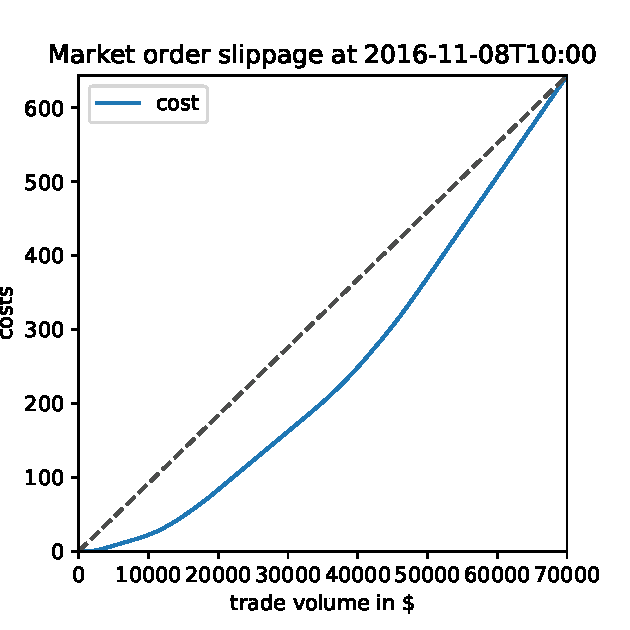
\includegraphics[width=0.3\textwidth]{content/drawings/nonlinearcosts}
	\caption{Non-linear slippage growth.}
	\label{fig:nonlinearcosts}
\end{wrapfigure}
While discretization of market variables mainly affects the strategies explanatory power, the resolution of private variable \lstinline!volume! leads to considerable rounding issues in regards to the cost function employed. As observed successor states $x_{t-1}$ must be discretized equally to allow looking up the corresponding minimal costs, the immediate costs, as computed in \Cref{eq:imcost}, must be scaled accordingly. Simply replacing \lstinline!volume_traded! with \lstinline!round(volume_traded)! falsifies the actual costs, as they correlate to the accomplished trade volume in an  unpredictable, non-linear manner as indicated in \Cref{fig:nonlinearcosts}. Nevmyvaka \etal \Cite{Nevmyvaka:2006} did not mention this problematic and presumably did not perform any cost scaling at all.

\begin{description}
\item[Potential Improvements]  A simple, but imprecise approach is to perform cost scaling, as described above. In general, this problem should be void, when function approximations are trained from the original float values, instead of rounded values.
\end{description}


\subsection{Markovian Assumption}
\label{chap:backwardalgorithm:discussion:markovianassumption}
The proposed backward algorithm assumes individual \lstinline!trading_periods! to be of an (approximately) Markovian nature. This is in fact not true, as the \ac{OTS}'s internal masterbook shape depends drastically from the preceding trade history.\\

\Cref{fig:differingmasterbooks} shows differing masterbook shapes, that can build the base of a simulated \lstinline!trading_period!, \eg if starting at $t=45min$ and a remaining trade volume of 17.500\$.

\ref{fig:differingmasterbooks:NoSim} shows the original orderbook, as if no orders had been matched by our strategy. This version of the masterbook is queried by the original backward algorithm, potentially resulting in more passive trading aggressions, as it does not account for the own impact on the market at all. \ref{fig:differingmasterbooks:SimEq} and \ref{fig:differingmasterbooks:SimMarketOrder} show two ideas, how the market impact can be incorporated. Both lead to different masterbook shapes and to different subsets of attainable prices.\\

\begin{figure}[ht]
	\centering
	\begin{subfigure}[t]{0.3\textwidth}
        		\centering
        		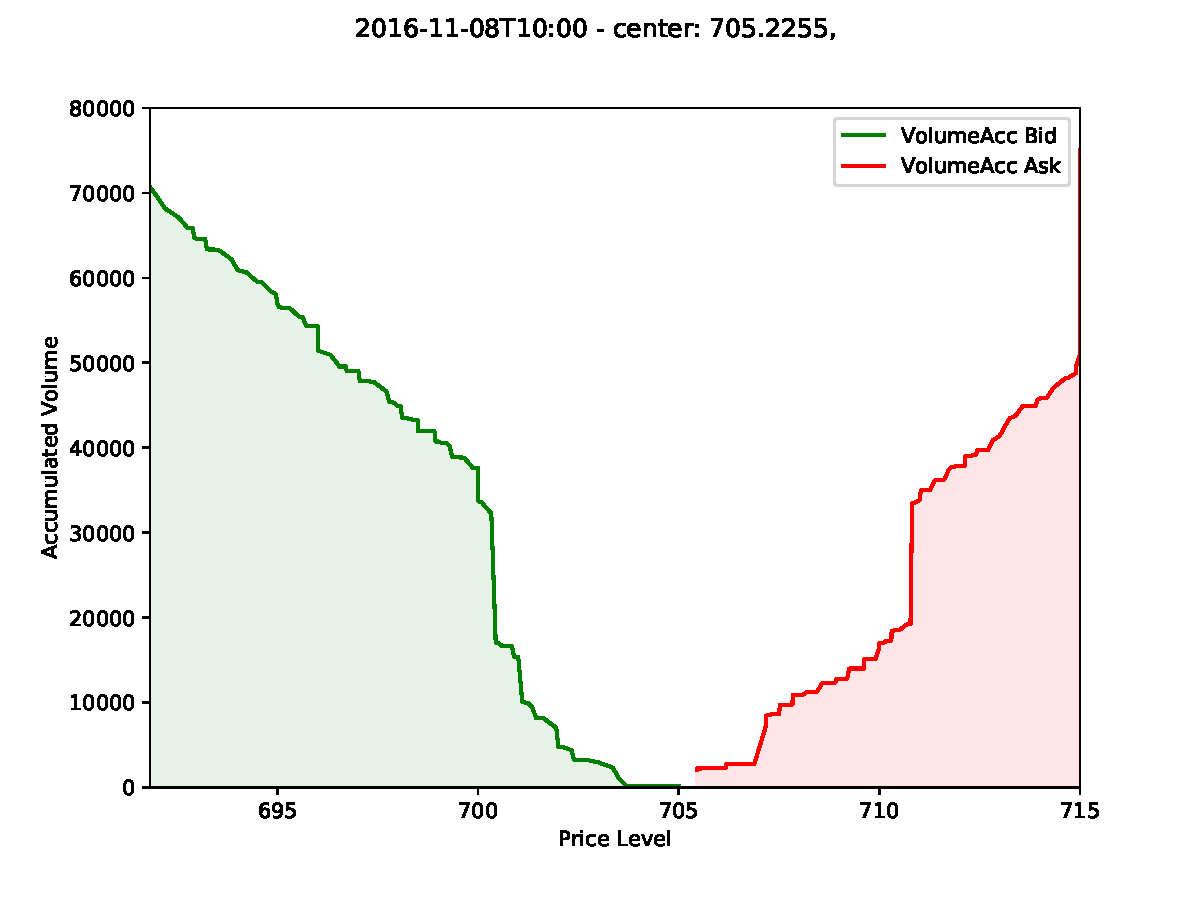
\includegraphics[width=\textwidth]{content/drawings/masterbook_customstart_NoSim}
        		\caption{Original Orderbook.}
		\label{fig:differingmasterbooks:NoSim}
    	\end{subfigure}
	\begin{subfigure}[t]{0.3\textwidth}
        		\centering
        		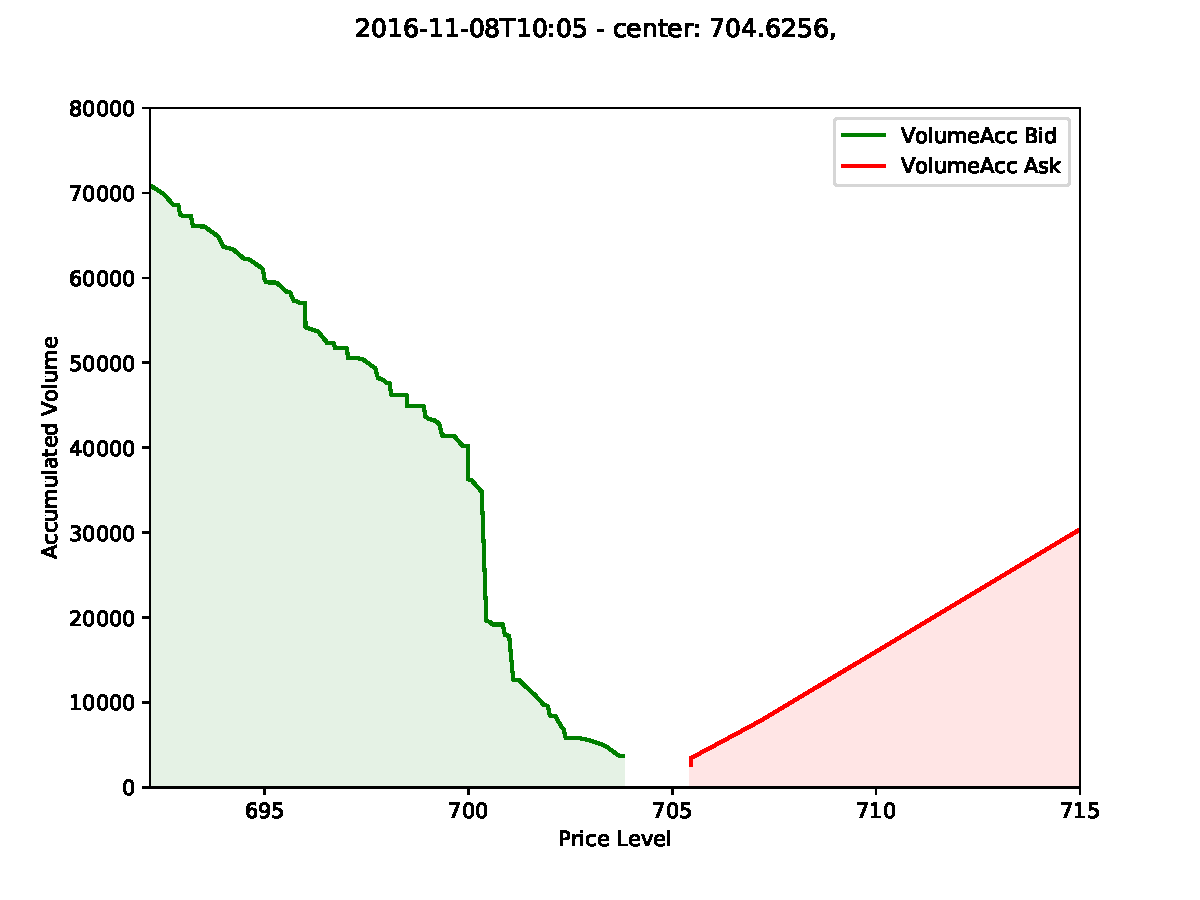
\includegraphics[width=\textwidth]{content/drawings/masterbook_customstart_SimMarketOrder}
        		\caption{Assuming 52.500 shares being matched at \lstinline!t=0!, then no further matches.}
		\label{fig:differingmasterbooks:SimMarketOrder}
    	\end{subfigure}%
	\begin{subfigure}[t]{0.3\textwidth}
        		\centering
        		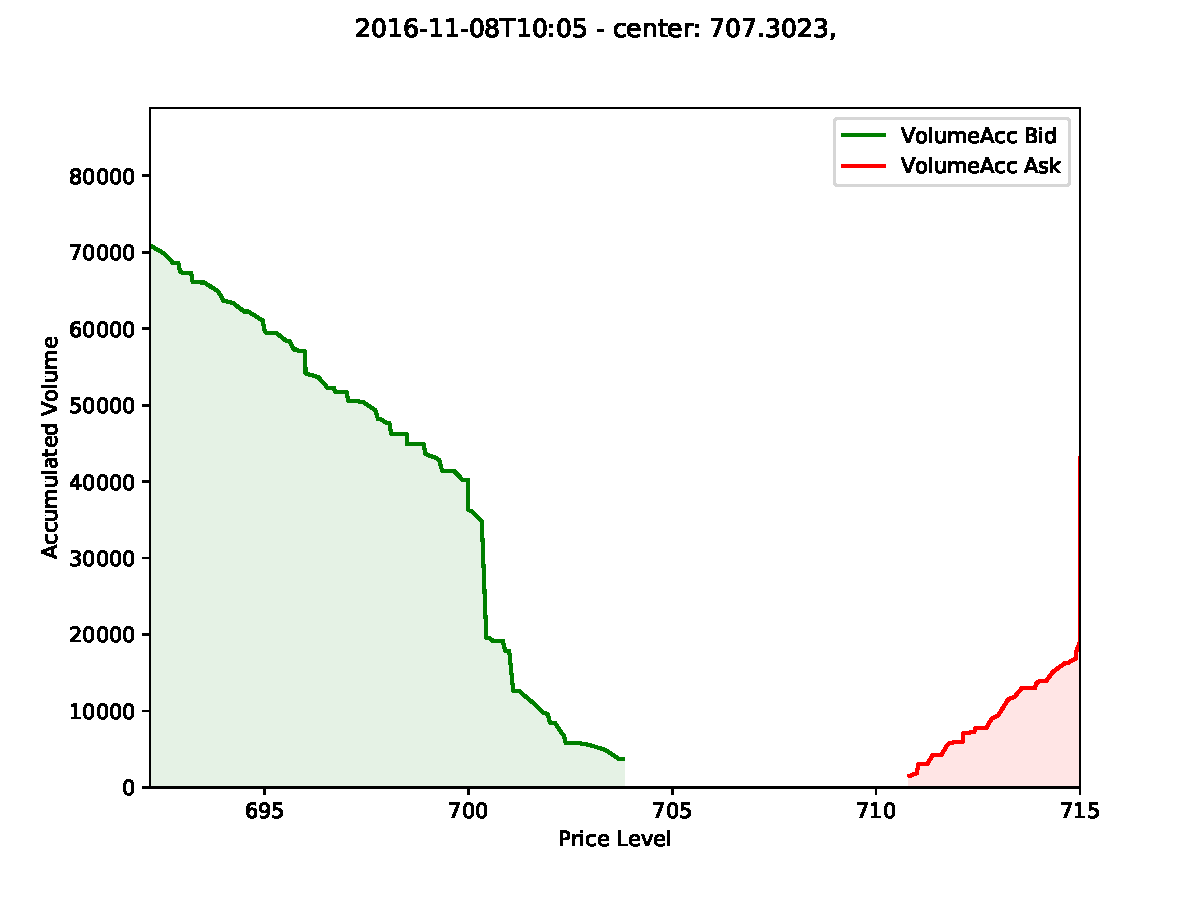
\includegraphics[width=\textwidth]{content/drawings/masterbook_customstart_SimEqual}
        		\caption{Assuming 52.500 shares being matched evenly at 1.166 shares per minute.}
		\label{fig:differingmasterbooks:SimEq}
    	\end{subfigure}%

	\caption{Different shaped masterbooks at \lstinline!t=45!.}
	The shapes differ, depending on the preceding trade history.
	\label{fig:differingmasterbooks}
\end{figure}

\begin{description}
\item[Potential Improvements] Initializing the \ac{OTS} outside the original start point ($t=0, V=100\%$), the supposedly traded volume must be incorporated, \eg as done in \Cref{fig:differingmasterbooks:SimEq}. Other than that, a more realistic sampling method may be applied: The forward sampling process, described in \Cref{chap:forwardlearning}, approaches sampling from the other side. Rather than evaluating actions on individual \lstinline!trading_periods!, the \ac{OTS} always starts with $V=100 \% $ and keeps going until the full trade is executed. As such, more realistic samples are generated. This does not give the problem a Markovian nature, but the internal masterbook is always of a realistic shape. In contrast to the backward approach, exhaustive exploration of the state space is not self-evident and must be enforced.
As a side benefit, the forward sampling approach generates more versatile samples for training the function approximates, as the generated samples do not necessarily start at \emph{discrete} start points only.
\end{description}



\subsection{Action Space}
\label{chap:backwardalgorithm:discussion:actionspace}
The mapping from actions to limits deserves some reflection as well. The proposed method (see \Cref{chap:actionspace}) adds the value of the chosen action directly to the current best price of the opposing book, such that the bid-ask spread must be crossed before any orders may be matched.\\

On the one hand, it seems pointless to fix the origin at the best price of the \emph{opposing} book. By doing so, it appears obvious, that decisions derived from state spaces including a variable for the current spread size, outperform decisions derived from state spaces not including this market variable. Indeed, the  bid-ask spread was posed as the market variable causing the greatest individual impact on cost reduction, namely -$7.97\%$, which is a major fraction of the maximum achievement of  $-12.85\%$\footnote{Strategies derived from five dimensional state spaces including the market variables Spread, ImmCost \& Signed Vol, as described in \Cref{chap:costs}, outperformed strategies derived from two dimensional state spaces, containing the private variables only, by $-12.85\%$ in average.}.\\

On the other hand, the proposed mapping method does not necessarily fit to the Bitcoin data at hand. As is shown in \Cref{fig:ploniexPriceHistory}, Bitcoin prices have burst from roughly 700\$ to more than 2.000\$ in the period of recording, \ie interpreting actions as the absolute difference to the current best prices, maps to significantly different levels of aggression as time passes.


\begin{description}
\item[Potential Improvements] lay in alternative action-limit mappings.\\
On the one hand side, the limit base may be fixed to the other side of the bid-ask-spread, reducing pointless dependencies on the speads size. On the other hand, actions should be interpreted as factors, rather than summands to allow for a consistent aggression interpretation. 
The mapping functions are thus redefined as follows:\\
\lstinline!limit_buy = ask * (1 + (a/1000))! instead of \lstinline!limit_buy = bid + a!\\
\lstinline!limit_sell = bid * (1 - (a/1000))! instead of \lstinline!limit_sell = ask - a!.

Actions $a$ now represent the deviation from the limit base in per mile. The influence of the chosen limit base is analyzed in \Cref{chap:exp:actionlimitmapping}.
\end{description}


\cleardoublepage{}